\section{SHA-1}
\textsc{SHA-1} was published in 1995 by the NIST as a standard, it is another hash algorithm, based on the Merkle-Damg\r{a}rd construction, which is widely implemented, though is deprecated as it is also considered cryptographically broken (see Chapter~\ref{chap:security}). It is still used due to legacy systems that do not have the support for SHA-2 or SHA-3.

SHA-1 pads the input message $M$, then splits it into $n$ blocs $M_1, M_2, {\ldots} ,M_n$ that are each $b=512$ bits long.
We shall focus here on the operations performed on a bloc $M_i$.
The compression function takes as an input a $512$-bit long message block and produces a $160$ bit long digest.

\subsection{Defining SHA-1 Constants And Functions}

\begin{itemize}
\item The \textsc{SHA-1} padding function pads the original message into $N=\vert M\vert_{512}$ consecutive blocs that are each 512 bits long: $M_0, M_1,{\ldots}, M_{N−1}$.

$$ M\vert \vert pad\lbrack 512\rbrack (\vert M\vert ) = M_0 \vert \vert M_1 \vert \vert \ldots \vert \vert M_{N-1}$$
\item A cyclic shift of x of k positions to the left is defined as:
$$RL(x,k)=(x<<k)\lor (x>>32-k)$$

\item Functions $F_0, {\ldots}, F_{79}$ are defined as follows:
\begin{equation}
F_t(B,C,D) =
\begin{cases}
(B \wedge C)  \vee (\overline{B} \wedge D) & \mbox{ for }0 \le t \le 19 \\
B \oplus C \oplus D & \mbox{ for } 20 \le t \le 39 \\
(B \wedge C)  \vee (B \wedge D)  \vee (C \wedge D) & \mbox{ for }40\le t\le 59 \\ 
B \oplus C \oplus D & \mbox{ for }60\le t\le 79 
\end{cases}
\end{equation}
Each function $F_t$ takes as inputs three 32-bit words and outputs one 32-bit word.

\item Constants $K_0, K_1, {\ldots}, K_{79}$, are defined as follows:
\begin{equation}
K_t =
\begin{cases}
\mbox{0x5a827999} & \mbox{ for }0 \le t \le 19 \\
\mbox{0x6ed9eba1} & \mbox{ for }20 \le t\le 39 \\ 
\mbox{0x8f1bbcdc} & \mbox{ for }40\le t\le 59 \\ 
\mbox{0xca62c1d6} & \mbox{ for }60\le t\le 79 
\end{cases}
\end{equation}
 \item The compression function iterates through 80 rounds for each input message bloc. Each one of these rounds performs the operations depicted in Figure~\ref{fig:SHA-1}
\end{itemize}

\begin{figure}[!ht]
        \centering
        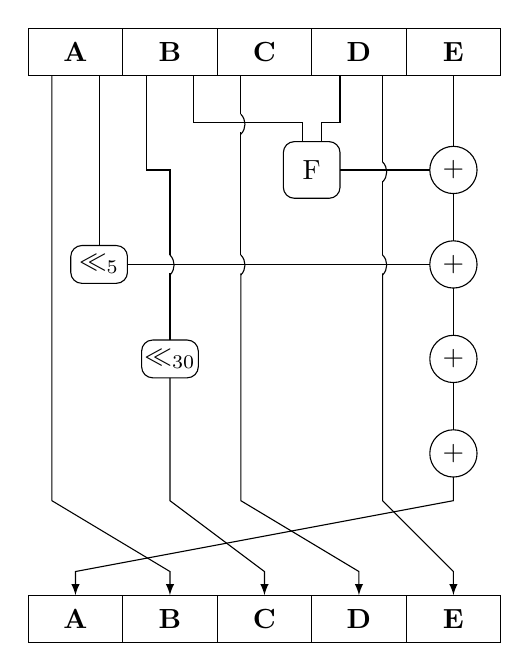
\begin{tikzpicture}[scale=1.2]
        %Box Messages
        \draw  (0,0) rectangle (1,0.5); \node [align=center] at (0.5,0.25){\textbf{A}};
        \draw  (1,0) rectangle (2,0.5); \node [align=center] at (1.5,0.25){\textbf{B}};
        \draw  (2,0) rectangle (3,0.5); \node [align=center] at (2.5,0.25){\textbf{C}};
        \draw  (3,0) rectangle (4,0.5); \node [align=center] at (3.5,0.25){\textbf{D}};
        \draw  (4,0) rectangle (5,0.5); \node [align=center] at (4.5,0.25){\textbf{E}};
        \draw  (0,6) rectangle (1,6.5); \node [align=center] at (0.5,6.25){\textbf{A}};
        \draw  (1,6) rectangle (2,6.5); \node [align=center] at (1.5,6.25){\textbf{B}};
        \draw  (2,6) rectangle (3,6.5); \node [align=center] at (2.5,6.25){\textbf{C}};
        \draw  (3,6) rectangle (4,6.5); \node [align=center] at (3.5,6.25){\textbf{D}};
        \draw  (4,6) rectangle (5,6.5); \node [align=center] at (4.5,6.25){\textbf{E}};
        %Cercles
        \draw  (4.5,5) circle (0.25); \node [align=center] at (4.5,5){+};
        \draw  (4.5,4) circle (0.25); \node [align=center] at (4.5,4){+};
        \draw  (4.5,3) circle (0.25); \node [align=center] at (4.5,3){+};
        \draw  (4.5,2) circle (0.25); \node [align=center] at (4.5,2){+};
        %Boxs + Textes
        \draw  [rounded corners] (2.7,4.7) rectangle (3.3,5.3); \node [align=center] at (3,5){F};
        \draw  [rounded corners] (0.45,3.8) rectangle (1.05,4.2); \node [align=center] at (0.75,4){$\ll_5$};
        \draw  [rounded corners] (1.2,2.8) rectangle (1.8,3.2); \node [align=center] at (1.5,3){$\ll_{30}$};
        %Traits et Fleches
        \draw [->, >=latex] (0.25,6) -- (0.25,1.5) -- (1.5,0.75) -- (1.5,0.5);
        \draw [-] (4.5,6) -- (4.5,5.25);\draw [-] (4.5,4.75) -- (4.5,4.25);\draw [-] (4.5,3.75) -- (4.5,3.25);\draw [-] (4.5,2.75) -- (4.5,2.25);\draw [->, >=latex] (4.5,1.75) -- (4.5,1.5) -- (0.5,0.75) -- (0.5,0.5);
        \draw [-] (1.25,6) -- (1.25,5) -- (1.5,5) -- (1.5,4.1);\draw [-] (1.5,3.905) -- (1.5,3.2);\draw [->, >=latex] (1.5,2.8) -- (1.5,1.5) -- (2.5,0.75) -- (2.5,0.5);
        \draw [-] (2.25,6) -- (2.25,5.59);\draw [-] (2.25,5.4) -- (2.25,4.1);\draw [->, >=latex] (2.25,3.905) -- (2.25,1.5) -- (3.5,0.75) -- (3.5,0.5);
        \draw [-] (3.75,6) -- (3.75,5.085);\draw [-] (3.75,4.88) -- (3.75,4.1);\draw [->, >=latex] (3.75,3.905) -- (3.75,1.5) -- (4.5,0.75) -- (4.5,0.5);
        \draw [-] (0.75,6) -- (0.75,4.2);\draw [-] (1.05,4) -- (4.25,4);
        \draw [-] (1.75,6) -- (1.75,5.5) -- (2.9,5.5) -- (2.9,5.3);\draw [-] (3.3,6) -- (3.3,5.5) -- (3.1,5.5) -- (3.1,5.3);\draw [-] (3.3,5) -- (4.25,5);
        %Arcs de cercle
        \draw (2.25,5.59) arc(45:-45:0.15cm);\draw (2.25,4.1) arc(45:-45:0.15cm);\draw (1.5,4.1) arc(45:-45:0.15cm);\draw (3.75,4.1) arc(45:-45:0.15cm);\draw (3.75,5.085) arc(45:-45:0.15cm);

        \end{tikzpicture}
        \caption{\label{fig:SHA-1}The $i^{th}$ round in SHA-1 $(0\le i \le 79)$.}
\end{figure}

\clearpage

\subsection{SHA-1 Algorithm}\label{section:sha1}
The pseudo-code for the SHA-1 algorithm is presented in Algorithm~\ref{algo:sha1}.

\begin{algorithm}[H]
\caption{SHA-1(x)}
\label{algo:sha1}
\begin{algorithmic}[1]
\State{\textbf{external procedures} SHA-1-\textsc{pad}}
\State{\textbf{global variables} $K_0, {\ldots},K_{79}$}
\State{$y \gets$ SHA-1-\textsc{pad} (x)}
\State{Define $y = M_1 \vert \vert M_2 \vert \vert \ldots \vert \vert M_N$, where each  $M_i$ is a 512-bit block.}
\State{$H_0 \gets \mbox{0x67452301}$}
\State{$H_1 \gets \mbox{0xefcdab89}$}
\State{$H_2 \gets \mbox{0x98badcfe}$}
\State{$H_3 \gets \mbox{0x10325476}$}
\State{$H_4 \gets \mbox{0xc3d2e1f0}$}
\For{$i \gets 1$ to $N$ }
\State{Define $M_i = W_0 \vert \vert W_1 \vert \vert \ldots \vert \vert W_{15}$, where each $W_j$ is a 32-bit word.}

\For{$t \gets 16$ to $79$ }
\State{$W_t \gets RL(W_{t-3}\oplus W_{t-8}\oplus W_{t-14}\oplus W_{t-16}, 1)$}
\EndFor{} 

\State{$A \gets H_0$}
\State{$B \gets H_1$}
\State{$C \gets H_2$}
\State{$D \gets H_3$}
\State{$E \gets H_4$}

\For{$t \gets 0$ to $79$ }
\State{$tmp \gets RL(A, 5) + f_t(B,C,D) + E + W_t + K_t$}
\State{$E \gets D$}
\State{$D \gets C$}
\State{$C \gets RL(B,30)$}
\State{$B \gets A$}
\State{$A \gets tmp$}
\EndFor{}

\State{$H_0 \gets H_0 + A$}
\State{$H_1 \gets H_1 + B$}
\State{$H_2 \gets H_2 + C$}
\State{$H_3 \gets H_3 + D$}
\State{$H_4 \gets H_4 + E$}
\EndFor{}

\Return{$H_0 \vert \vert H_1 \vert \vert H_2 \vert \vert H_3 \vert \vert H_4$}
\end{algorithmic}
\end{algorithm}

\clearpage
